% ---- Modele TP PC V2 -----------
\documentclass[a4paper,9pt,french]{scrartcl}
\usepackage[T1]{fontenc}%---pour l'encodage d'entr\'ee
\usepackage{array}%---pour les tableaux
\usepackage{titlesec}%---modification des titres
\usepackage{ulem}%---pour le soulignage
\usepackage[dvipsnames]{xcolor}%---pour avoir d'autres couleurs
\usepackage{color}%---pour avoir les couleurs de base
\usepackage{babel}%---pour les trucs de langue et la francisation

\usepackage{graphicx}%----pour mettre des images
\usepackage[utf8]{inputenc}%---encodage
\usepackage{geometry}%---pour modifier les tailles et mettre a4paper
%\usepackage{awesomebox}%---pour les boites d'exercices, de pbq et de croquis ---d\'esactiv\'e pour les TP de PC
\usepackage{tikz}%---pour dessiner + d\'ependance de chemfig
%\usepackage{tabularx}%---pour dimensionner automatiquement les tableaux avec variable X
\usepackage{fancyhdr}%---pour les en-t\^ete personnalis\'ees
\usepackage{blindtext}%---pour les liens
\usepackage{hyperref}%---pour les liens (\`a mettre en dernier)
\usepackage{caption}%---pour la francisation de la l\'egende table vers Tableau
 \usepackage{float}% --- pour placer les figures et tableaux où l'on souhaite avec argument H
 \usepackage{multicol}
 \usepackage{amsmath}
 \usepackage{geometry}
 \geometry{vmargin=2.5cm}

\captionsetup{labelfont=sc}%---pour la francisation de la l\'egende table vers Tableau
\def\frenchtablename{Tableau}%---pour la francisation de la l\'egende table vers Tableau
\pagestyle{fancy}
\renewcommand\headrulewidth{1pt}
\fancyhead[L]{TP 6}
\fancyhead[R]{Saux Paulhenry}
\title{Compte rendu de TP 6}
\date{}
\author{}

\geometry{a4paper}
% ----------- Création des commandes de couleur ----------
\makeatletter
\newcommand{\coloruline}[2]{%
        \UL@protected\def\temp@uline{\leavevmode \bgroup
            \markoverwith{\textcolor{#1}{\rule[-0.5ex]{2pt}{0.4pt}}}%
        \ULon}%
        \temp@uline{#2}%
    }

    \newcommand{\coloruuline}[2]{%
        \UL@protected\def\temp@uuline{\leavevmode \bgroup
            \UL@setULdepth
            \ifx\UL@on\UL@onin \advance\ULdepth2.8\p@\fi
            \markoverwith{\textcolor{#1}{\lower\ULdepth\hbox
                {\kern-.03em\vbox{\hrule width.2em\kern1\p@\hrule}\kern-.03em}}}%
        \ULon}%
        \temp@uuline{#2}%
    }

\makeatother

\renewcommand{\thesection}{\arabic{section}}
\renewcommand{\thesubsection}{\arabic{subsection}}
\renewcommand{\thesubsubsection}{\arabic{subsubsection}}
\begin{document}
% ---------------- Modification des titres de niveau 1,2 et 3 --------------------
\titleformat
{\section} % command
%[display] % shape
{\Large} % format
{\coloruuline{red}{\thesection. }} % label
{0ex} % sep
{\coloruuline{red}} % before-code
[] % after-code

\titleformat
{\paragraph} % command
%[display] % shape
{\Large} % format
{\coloruline{NavyBlue}{\theparagraph. }} % label
{0ex} % sep
{\coloruline{NavyBlue}} % before-code
[] % after-code

\titleformat
{\subsection} % command
%[display] % shape
{\Large} % format
{\coloruline{red}{\thesection.\thesubsection. }} % label
{0ex} % sep
{\coloruline{red}} % before-code
[] % after-code

\titleformat
{\subsubsection} % command
%[display] % shape
{\large} % format
{\coloruline{ForestGreen}{\thesection.\thesubsection.\thesubsubsection. }} % label
{0ex} % sep
{\coloruline{ForestGreen}} % before-code
[] % after-code

\titleformat
{\chapter} % command
%[display] % shape
{\large} % format
{\coloruline{NavyBlue}{\thechapter \:- }} % label
{0ex} % sep
{\coloruline{NavyBlue}} % before-code
[] % after-code


% ---------------- Début du corps du document ------------------------------------

\section{Introduction}
\subsection{Objectifs}
Nous souhaitons étudier le phénomène de résonnance dans des systèmes oscillants. Nous nous appuyrons sur une étude électrocinétique, en particulier un circuit RLC série en régime sinusoidal en régime forcé. Ce type de circuit nous permet d'étudier une résonnance en charge (par l'analyse de la tension aux bornes du condensateur) ou en intensité (par l'analyse de la tension aux bornes de la résistance).
\subsection{Sommaire}
Ce TP se décompose en quatre parties :
\begin{enumerate}
 \item Analyse qualitative de la tension aux bornes de la résistance
 \item Étude de la résonnance en intensité
 \item Analyse qualitative de la tension aux bornes du condensateur
 \item Étude de la résonnance en charge
\end{enumerate}
\section{Protocole}
Dans toute ce TP, nous paramétrons le générateur pour fournir un signal sinusoidal d'amplitude 2.0 V crète à crète.
\subsection{Analyse qualitative de la tension aux bornes de la résistance \& Étude de la résonnance en intensité}
\subsubsection{Matériel}
\begin{itemize}
 \item Bobine Leybold de 36mH, 9.5 \(\Omega\) et 1000 spires
 \item Générateur Basse Fréquence délivrant un signal sinusoidal
 \item Résistance de \(5\omega\)
 \item Un oscilloscope comportant 2 canaux
 \item C\^ables
\end{itemize}
\subsubsection{Description du montage expérimental}
Nous réalisons le montage indiqué en figure 1. Par convention, on associe la mesure de la tension du générateur au canal 1 et celle de la résistance au canal 2.
\begin{center}
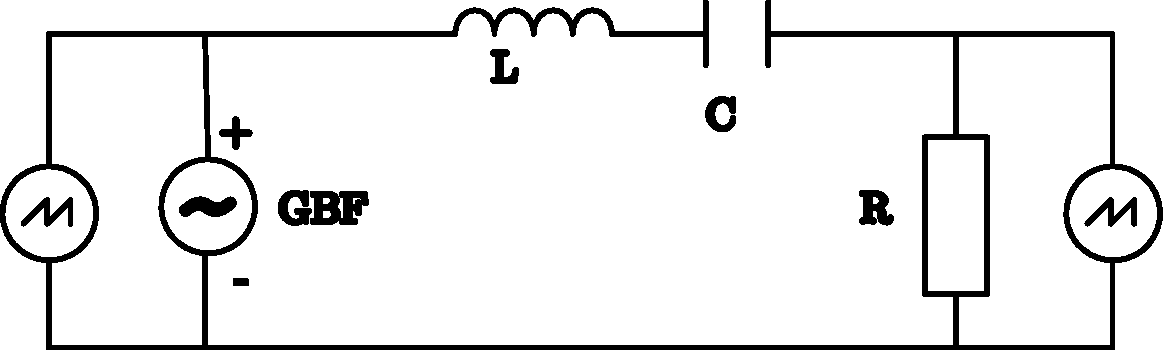
\includegraphics[scale=0.3]{circuit1}
\end{center}
\subsubsection{Mesures à effectuer}
\paragraph{Étude qualitative}
Pour une fréquence proche de la fréquence de résonnance, une fréquence haute et une basse fréquence :
\begin{enumerate}
\item Relever l'amplitude tension du générateur et celle de la résistance
\item Relever la phase de tension du générateur et celle de la résistance
\end{enumerate}
\paragraph{Mesure de la fréquence de résonnance}
\begin{enumerate}
\item Paramétrer le générateur sur la fréquence de résonnance théorique
\item Paramétrer l'oscillateur sur le mode XY Display
\item Modifier la fréquence du générateur pour que l'ellipse affichée devienne une droite et relever la valeur de fréquence
\end{enumerate}
\paragraph{Mesures des valeurs du diagramme de Bode}
Le diagramme de Bode synthétise les informations sur l'amplitude des tensions et sur le déphasage.
\begin{enumerate}
 \item Se placer sur le mode par defaut de l'oscillateur
 \item Pour 6 valeurs (par pas de 10 Hz environ) de fréquence au-dessus de la fréquence de résonnnace, relever la tension du générateur et de la résistance
  \item Pour 6 valeurs (par pas de 10 Hz environ) de fréquence au-dessous de la fréquence de résonnnace, relever la tension du générateur et de la résistance
  \item Pour 6 valeurs de fréquence autour de la fréquence de résonnance, relever le déphasage.
\end{enumerate}

\subsection{Analyse de la tension aux bornes du condensateur \& Étude de la résonnance en charge}
\subsubsection{Matériel}
\begin{itemize}
 \item Bobine Leybold de 36mH, 9.5 \(\omega\) et 1000 spires
 \item Générateur Basse Fréquence délivrant un signal sinusoidal
 \item Résistance de \(5\omega\) et de \(50\omega\)
 \item Un oscilloscope comportant 2 canaux
 \item C\^ables
\end{itemize}
\subsubsection{Description du montage expérimental}
Nous réalisons le montage indiqué en figure 2. Par convention, on associe la mesure de la tension du générateur au canal 1 et celle du condensateur au canal 2.
\begin{center}
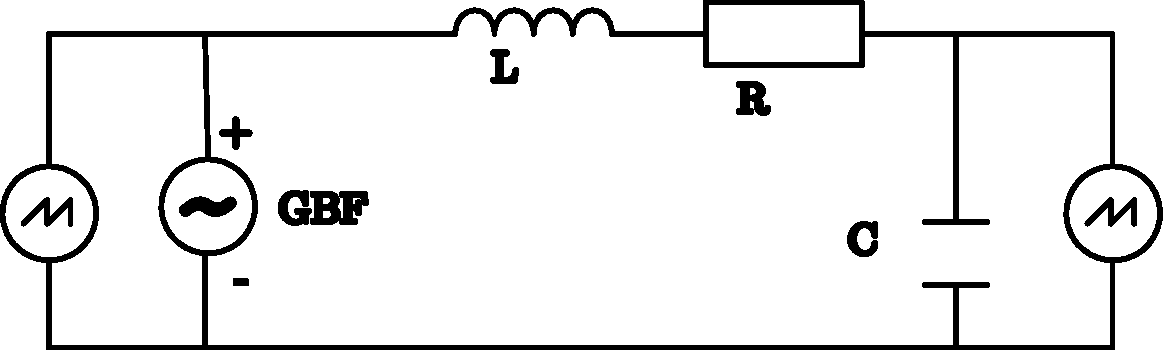
\includegraphics[scale=0.3]{circuit2}
\end{center}
\subsubsection{Mesures à effectuer}
\paragraph{Étude qualitative}
Pour une fréquence proche de la fréquence de résonnance, une fréquence haute et une basse fréquence :
\begin{enumerate}
\item Relever l'amplitude tension du générateur et celle du condensater
\item Relever la phase de tension du générateur et celle du condensater
\end{enumerate}
\paragraph{Mesures de l'amplitude}
\begin{enumerate}
 \item Se placer sur le mode par defaut de l'oscillateur
 \item Pour 6 valeurs (par pas de 10 Hz environ) de fréquence au-dessus de la fréquence de résonnnace, relever la tension du générateur et de la résistance
  \item Pour 6 valeurs (par pas de 10 Hz environ) de fréquence au-dessous de la fréquence de résonnnace, relever la tension du générateur et de la résistance
  \item Recommencer les 2 étapes précédentes avec une résistance de 50 \(\omega\)
\end{enumerate}
\section{Mesures}
\subsection{Analyse qualitative de la tension aux bornes de la résistance \& Étude de la résonnance en intensité}
\subsubsection{Analyse qualitative}
\begin{center}
\begin{tabular}{llll}
Fréquence & Basse & Résonnnance & Haute\\
Tension du générateur (V) & 1,972 & 1,972 & 1,972\\
Tension de la résistance & très faible \(\simeq 100 \mu V\) & la plus haute \(\simeq 600 mV\) & très faible \(\simeq 100 \mu V\)\\
Déphasage & \(-\frac{\pi}{2}\) &  0 &  \(+\frac{\pi}{2}\)
\end{tabular}
\end{center}
\subsubsection{Analyse quantitative}
\paragraph{Données}
\begin{center}
\begin{tabular}{lll}
Fréquence (Hz) & Tension du générateur (Ue) (V) & Tension de la résistance (Ur) (mV)\\
100 & 1,972 & 1,19\\
269 & 1,972 & 14\\
426 & 1,992 & 23\\
578 & 1,992 & 33\\
730 & 1,992 & 37\\
1140 & 1,972 & 339\\
1150 & 1,972 & 386\\
1160 & 1,952 & 434\\
1170 & 1,932 & 515\\
1180 & 1,932 & 575\\
1190 & 1,932 & 630\\
1200 & 1,932 & 640\\
1211 & 1,932 & 611\\
1221 & 1,932 & 548\\
1231 & 1,932 & 487\\
1241 & 1,932 & 424\\
1251 & 1,952 & 378\\
1261 & 1,972 & 334\\
1271 & 1,972 & 301\\
1794 & 1,992 & 36,2\\
1947 & 1,992 & 38,5\\
2100 & 1,992 & 31,0\\
5418 & 1,992 & 10,4
\end{tabular}
\end{center}
\begin{center}
\begin{tabular}{ll}
Fréquence (Hz) & Décalage (rad)\\
1050 & -1,57 (\(-\frac{\pi}{2}\))\\
1146 & -0,785 (\(-\frac{\pi}{4}\))\\
1197 & 0\\
1237 & 0,785 (\(\frac{\pi}{4}\))\\
1389 & 1,57 (\(\frac{\pi}{2}\))
\end{tabular}
\end{center}
\begin{center}
\begin{tabular}{lll}
Fréquence de résonnance & Fréquence Haute & Fréquence Basse\\
1199 & 1997 & 1200
\end{tabular}
\end{center}
\paragraph{Incertitudes}
L'incertitude liée aux valeurs d'amplitude obtenues est liée à la précision des appareils de mesures. On a donc :
\[u(U_r) = \frac{1}{\sqrt{3}}mV, u(U_e) = \frac{0.001}{\sqrt{3}}V, u(f) = \frac{1}{\sqrt{3}}Hz\]

Celle sur le déphasage est elle aussi liée à la précision de l'appareil de mesure, ici l'échelle horizontale et de sa graduation utilisée par l'oscilloscope. C'est pourquoi nous avons plutot chercher à obtenir des valeurs de fréquence pour lesquelles les décalages entre courbes sont faciles à lires, c'est à dire des décalages multiples de \(\frac{\pi}{4}\). De cette façon, il plus facile de vérifier si les courbes sont en quadrature de phase ou en opposition de phase et de relever la valeur de fréquence associée. L'incertitude liée au décalage de phase est dès lors considérée comme négligeable devant celle liée à la fréquence. On a donc : \[u(f) = \frac{1}{\sqrt{3}}Hz\]

L'incertitude liée à la fréquence de résonnance est liée à l'échelle utilisée par l'oscilloscope pour afficher l'ellipse. Pour l'évaluer correctement, nous mesurer la fréquence la plus haute et la plus basse pour lesquelles on peut considérer l'ellipse comme une droite. On obtient alors \[f_r = (1199\pm1.5)Hz\]
\subsection{Analyse de la tension aux bornes du condensateur \& Étude de la résonnance en charge}
\subsubsection{Données}
\subsubsection{Analyse qualitative}
\begin{center}
\begin{tabular}{llll}
Fréquence & Basse & Résonnnance & Haute\\
Tension du générateur (V) & 1,972 & 1,972 & 1,972\\
Tension du condensateur (V) & \(\simeq 2 \) & la plus haute \(\simeq 34\) & très faible \(\simeq 400 \mu V\)\\
Déphasage & 0 & \(-\frac{\pi}{4}\) &  \(-\pi\)
\end{tabular}
\end{center}
\subsubsection{Analyse quantitative}
\begin{center}
\begin{tabular}{lll}
Fréquence & Tension du générateur (Ve) (V) & Tension du condensateur (Vs) (V)\\
1130 &2.0 & 17\\
1146 &2.0 & 20,6\\
1156 &2.0 & 24\\
1166 &2.0 & 27\\
1176 &2.0 & 31\\
1186 &2.0 & 33\\
1196 &2.0 & 36\\
1206 &2.0 & 34\\
1216 &2.0 & 31\\
1226 &2.0 & 27\\
1236 &2.0 & 24
\end{tabular}
\end{center}
\begin{center}
\begin{tabular}{lll}
Fréquence (Hz) & Tension du générateur (Ve) (V) & Tension du condensateur (Vs) (V)\\
13 & 2,3 & 0,690\\
824 & 2,3 & 4,32\\
880 & 2,3 & 4,82\\
925 & 2,3 & 5,50\\
981 & 2,3 & 6,50\\
1020 & 2,3 & 7,34\\
1072 & 2,3 & 8,65\\
1100 & 2,3 & 9,41\\
1120 & 2,3 & 9,99\\
1180 & 2,3 & 10,3\\
1220 & 2,3 & 9,47\\
1232 & 2,3 & 9,50\\
1246 & 2,3 & 8,81\\
1350 & 2,3 & 5,60\\
1400 & 2,3 & 4,65\\
1450 & 2,3 & 4,00
\end{tabular}
\end{center}
\subsubsection{Incertitude}
Les incertitudes sont les m\^emes que pour la partie précédente.
\section{Graphiques}
\subsection{Analyse de la tension aux bornes de la résistance \& Étude de la résonnance en intensité}
\begin{figure}[H]
 \begin{center}


\includegraphics[scale=0.4]{1}
 \end{center}
\caption{Diagramme de Bode en amplitude}
\end{figure}
\begin{figure}[H]
 \begin{center}


\includegraphics[scale=0.4]{2}
 \end{center}
\caption{Diagramme de Bode en déphasage pour \(\Delta \phi = \phi_{e}-\phi_{r}\)}
\end{figure}
\subsection{Analyse de la tension aux bornes du condensateur \& Étude de la résonnance en charge}
\begin{figure}[H]
 \begin{center}


\includegraphics[scale=0.4]{3}
 \end{center}
\caption{Diagramme de Bode en amplitude pour \(R=5\Omega\)}
\end{figure}
\begin{figure}[H]
 \begin{center}


\includegraphics[scale=0.4]{4}
 \end{center}
\caption{Diagramme de Bode en amplitude pour \(R=50\Omega\)}
\end{figure}
\section{Exploitation des résultats}
\subsection{Analyse de la tension aux bornes de la résistance \& Étude de la résonnance en intensité}
\subsubsection{Analyse qualitative}
La fonction de transfert $H_c = \frac{\underline{U_r}}{\underline{U_e}}$ est donnée par :
\begin{equation}
H_c(\omega) = \frac{R}{R + j\left(L\omega - \frac{1}{C\omega}\right)}
\end{equation}
et
\begin{equation}
\tan(\varphi) = \frac{-(L\omega - \frac{1}{C\omega})}{R}
\end{equation}
On peut calculer le déphasage et l'amplitude de \(U_r\) selon les valeurs de fréquence :
\begin{itemize}
    \item \textbf{Basse Fréquence ($\omega \to 0$)} :  Le module $|H_c| \to 0$. $\underline{U_r}$ est très faible et le déphasage tend vers $+\frac{\pi}{2}$.
    \item \textbf{Haute Fréquence ($\omega \to \infty$)} : Le module $|H_c| \to 0$. $\underline{U_r}$ est très faible et le déphasage tend vers $-\frac{\pi}{2}$.
    \item \textbf{Résonance ($\omega = \omega_0$)} : L'impédance est minimale lorsque $L\omega_0 = \frac{1}{C\omega_0}$, soit $\omega_0 = \frac{1}{\sqrt{LC}}$. $|H_c| = \frac{R}{R_{tot}}$ est maximal. Le déphasage est nul.
\end{itemize}
Les prédictions correspondent bien aux observations. En effet, pour le déphasage, nous avons relevé la valeur de \(\Delta \phi = \phi_{e}-\phi_{r}\), alors que les valeurs de déphasage calculées correspondent à \(\Delta \phi = \phi_{r}-\phi_{e}\), soit l'opposé. Il est donc normal qu'on trouve les valeurs prédites, mais au signe près. Il s'agit du comportement d'un filtre passe-bande.
\subsubsection{Analyse quantitative}
Le but est de déterminer expérimentalement les valeurs du facteur de qualité et de la fréquence de résonnance. Avec EQ1, On sait que
\begin{equation}
Q = \frac{1}{R}\sqrt{\frac{L}{C}}
\end{equation}
et
\begin{equation}
\omega_r = \frac{1}{\sqrt{LC}2\pi}
\end{equation}
Avec EQ 1, on sait que
\begin{equation}
\frac{V_s}{V_e} = (1+Q^2(\frac{f}{f_r}-\frac{f_r}{f})^2)^{-1/2}
\end{equation}
En traçant $\frac{V_s}{V_e}$ en fonction de la fréquence, on peut déduire ces 2 paramètres. Avec Regressi, on obtient\footnote{Nous avons du rajouter un coefficient multiplicateur à l'expression utilisée pour obtenir une modélisation plus proche des données.} :
\[Q=(16,56\pm0,17), f_r=(1,19853 \pm 0,00024)\cdot 10^{3} Hz\]
Les valeurs obtenues sont assez proche des valeurs théoriques calculées :
\[Q = 18.5 , f_r = 1186\]

La valeur de fréquence de résonnance la plus proche est celle obtenue avec la méthode par regression, bien que la seconde méthode soit plus rapide à mettre en oeuvre et produise tout de m\^eme un résultat similaire. %TODO

La différence de facteur de qualité peut s'expliquer par la résistance des fils, et résistances internes du générateur et des appareils de mesure que nous avons négligés. Comme les résistances utilisées sont faibles \(\simeq 10 \Omega\), ces dernières peuvent ne plus \^etre négligées.
Le diagramme de Bode en déphasage est également celui attendu et prédit par l'analyse qualitative.
\subsection{Analyse de la tension aux bornes du condensateur \& Étude de la résonnance en charge}
\subsubsection{Analyse qualitative}
On déduit de la fonction de transfert l'amplitude :
\begin{equation}
 |H_c(f)| = \frac{1}{\sqrt{\left(1 - \frac{f^2}{f_0^2}\right)^2 + \left(\frac{f}{f_0 Q}\right)^2}}
\end{equation}
On déduit de la fonction de transfert son argument :
$$\phi(f) = - \text{Arg}(Z)$$

Pour un nombre complexe $Z = X + jY$, l'argument est $\text{Arg}(Z) = \arctan\left(\frac{Y}{X}\right)$.
Ici, $X = 1 - \frac{f^2}{f_0^2}$ et $Y = \frac{f}{f_0 Q}$.

Donc, le déphasage $\phi(f)$  est :

$$\phi(f) = - \arctan\left(\frac{\frac{1}{Q} \frac{f}{f_0}}{1 - \left(\frac{f}{f_0}\right)^2}\right)$$

On peut calculer le déphasage et l'amplitude de \(U_r\) selon les valeurs de fréquence :
\begin{itemize}
    \item \textbf{Basse Fréquence ($f \to 0$)} :  Le module $|H_c| \to 1$. $|U_r| = |E|$. De plus, \(\phi(f) \to - \arctan(0) = 0\), donc le déphsage est nul.
    \item \textbf{Haute Fréquence ($f \to \infty$)} : Le module $|H_c| \to 0$. $|U_r|$ est très faible. Pour l'argument, celui-ci doit tendre vers \(-\pi\)
    \item \textbf{Résonance ($f = f_0$)} : $|H_c| = Q$. On en déduit que $|v_s| = Q \cdot |v_e|$. De plus, $\phi(f_0) = - \arctan(\infty) = -\frac{\pi}{2}$
\end{itemize}
Calcul de l'argument à haute fréquence :

Pour un grand $f$, $Y/X \approx \frac{f/(f_0 Q)}{-f^2/f_0^2} = - \frac{f_0}{f Q} \to 0^-$.

L'argument de l'arctangente est négatif et très petit, mais comme $f/f_0 > 1$, la fonction est définie par $Y/(|X|)$ avec une correction de $\pi$ pour l'argument de $Z$. Or, $\text{Arg}(Z) = \arctan\left(\frac{Y}{X}\right)$ se trouve dans le deuxième quadrant (Réel $X<0$, Imaginaire $Y>0$), donc $\text{Arg}(Z) \to \pi$.

Donc $$\phi(f) \to - \pi $$

Les prédictions correspondent bien aux observations.
%Expression et limites qui confrirment nos résultats
\subsubsection{Analyse quantitative}
On sait que
\begin{equation}
 \frac{V_s}{V_e} = \frac{1}{1-\frac{f^2}{f_0^2}+j\frac{f}{f_0Q}}
\end{equation}
On  peut donc déduire \(Q\) et \(f_0\) des mesures effectuées.

On sait aussi que \(\omega_r = \omega_0\sqrt{1-\frac{1}{2Q^2}}\). De plus, l'expression du facteur de qualité est \[Q = \frac{\sqrt{LC}}{RC}\]
\paragraph{R = 5 \(\Omega\)}


Dans le cas où on choisit \(R=5\Omega\), le facteur de qualité obtenu sera très grand et \(f_0 \simeq f_r\). Avec Regressi, on obtient \(f_0 = (1,19738 \pm 0,00068)\cdot 10^3\text{ Hz}, Q = (17,90 \pm0,18) \), ce qui est cohérent avec les valeurs théoriques (\(Q = 18.50, f_0 = f_r = 1186 \text{ Hz}\)).

\paragraph{R = 50 \(\Omega\)}
Avec \(R = 50 \Omega\), on ne peut plus négliger le terme \(\frac{1}{2Q^2}\) et on a bien \(\omega_r = \omega_0\sqrt{1-\frac{1}{2Q^2}}\).

Regressi donne $f_0=(1,17657 \pm0,00094)\cdot 10^3 \text{ Hz}, Q=(4,483 \pm0,044)$, ce qui correspond aux valeurs prévues : \(f_r = 1175 \text{ Hz}, Q = 4.50\)


On remarque que plus la résistance est élevée, plus le facteur de qualité est faible, et donc moins le phénomène de résonnance sera important.
\section{Conclusion}
Les analyses qualitatives et quantitatives ont confirmé les prédictions théoriques issues de l'étude des fonctions de transfert pour chaque configuration.
Pour la première configuration, les mesures ont mis en évidence le comportement de ce circuit comme un filtre passe-bande.

Les valeurs expérimentales sont cohérentes avec les valeurs théoriques. L'écart sur le facteur de qualité est probablement dû à la négligence des résistances internes des appareils et des fils de connexion.

La tension aux bornes du condensateur de la deuxième configuration présente une résonance en charge.

De plus, l'influence de la résistance a été démontré. Ainsi, pour \(R=5\Omega\), le facteur de qualité est élevé alors que pour \(R=50\Omega\), le facteur de qualité est faible et la fréquence de résonance \(f_r\) est légèrement inférieure à la fréquence \(f_0\).
\end{document}
